\chapter{State-of-the-Art} \label{chap:chap2}

\section*{}

Social networks are changing the paradigm of communication between people. We have seen an increasing growth of the number of people using them in the past few years, and the same applies for the amount of time spent by people in these communities. This popularity brings a huge potential to these platforms, for instance, for promoting or marketing of products, sharing various kinds of information, and stimulating the collaboration among its users.
Using this strong sharing component, and with the help of some other features for communication between people, such as chat, instant messaging, video-conferencing and so on, these platforms develop some features of collaborative environments, making them attractive to implement the concept of Collective Intelligence \cite{kn:CSV11}. 

The fact that we can use a communication network everywhere these days had an impact on the social networks growth, popularity, and volume of information shared. To be online anywhere and at any moment, has become an habit for millions of human beings, and the smartphones' expansion had a great contribution to that. 
However, their increasing popularity does not exactly mean that people are easily driven or compelled to use new ones. Instead, they usually get bored faster and their acceptance of different networks and environments diminishes. 

So, in order to succeed, a new player, in this case, a new social network or platform, has to find new ways in order to keep people addicted to their services, and attract even more people.  We will start by clarifying some concepts that are in some way related with the project.

\section{Online Collaboration Tools}\label{sec:onlinecol}

Nowadays, we have a wide range of tools we can use to perform some kind of online collaboration, such as real-time collaborative text editors (Google Drive, for instance), wikis, Q\&A websites (\emph{StackOverflow and SuperUser} have an enormous success inside the IT community, allowing people to ask questions and to say problems they're facing and see them answered by someone with expertise on the field), and so on.

Most of these platforms, and their success, rely heavily on their number of users, on their features, and on the information flow generated and shared by them. In cases where the shared information is made public (Q\&A websites, for instance), the "community sense" perceived by the user, along with the value of the existing information, is fundamental to the acceptance of the platform.

That kind of collaboration lies deeply within the concept of Collective Intelligence, emerged from the debates held by Pierre Lévi \cite{kn:Le98}, where it is assumed that the intelligences of each individual are added and shared by the society.

\begin{quote}
"What is collective intelligence? It is a form of universally distributed intelligence, constantly enhanced, coordinated in real-time, and resulting in the effective mobilization of skills... My initial premise is based on the notion of a universally distributed intelligence. No one knows everything, everyone knows something, all knowledge resides in humanity." 
\end{quote}

This is something meant to be explored deeply in this thesis and the concept behind it, due to the functionality and usability the application aims to give to the passengers, in order to keep them generating useful information for other users.

The growth of online collaboration lead also to the growth of a new business model, called \emph{crowdsourcing}, where people submit problems to a community , instead of solving them on their own, hoping for the community to reply with better and/or more creative solutions.

That business model has also evolved into several sub-types, such as \emph{crowdfunding}, where someone prompts the community with a solution for a problem and asks the members of the community for funding, in order to develop and launch said solution, if the said members think the solution is viable, creative and/or necessary.

\section{Mobile Environment Overview}\label{sec:mobove}

As said before. we live in an era where smartphones allowed us to take advantages of the massification of wireless networks in order to be online, anywhere and at any given time.

They also allowed us to perform tasks we didn't imagine ourselves performing from a mobile phone twenty years ago, such as:

\begin{itemize}
\item Reading our e-mail account and send new e-mails.
\item Navigating on websites.
\item Share photos with friends via messages or social networks.
\item 'Check-in' at restaurants, clubs, museums, etc.
\item Use native applications to fetch several types of information: news, weather information, football scores, and even \emph{public transport information}, such as schedules.
\end{itemize}

The appearance of mobile operating systems with high number of default functionalities, such as Android \footnote{\url{http://www.android.com/meet-android/}} (maintained by Google) or iOS \footnote{\url{https://www.apple.com/ios/}} (from Apple Company), allied to the easy development of native applications for those OS's, lead to an exponential growth in the number of that type of devices worldwide and thus, their native applications.

Android is, by far, the mobile operating system with most devices sold and has a steep growing trend. It is known for being an open source Linux-based system, suitable for both smartphones and tablets and very flexible concerning to hardware configurations.

It has been well received by third-party phone manufacturers, and it has a large community of developers, as well as millions of native applications available for download. Users can find these application in their official store, \emph{Google Play Store}, the largest app store worldwide \cite{kn:Are13}, or through third-party websites.

Apple's iOS, however, is a closed-source system, for installation on Apple's devices only. 
It was originally developed for Apple's smartphones, iPhone, but it has since then been extended to other devices from the company, such as tablets (iPad) or portable music players (iPod Touch). Its application store is the most profitable worldwide.

Both Android and iOS have evolved since their first versions, not only adding functionality and features, but also providing developers with new methods to make their applications more usable, efficient and aesthetically attractive.

Mobile devices who have these operative systems are also equipped with a lot of embedded sensors, that provide help and data to some features of applications. Some of these sensors are:

\begin{itemize}
\item Motion Sensors (accelerometers, gyroscopes, gravity sensors);
\item Environmental Sensors (barometers, thermometers);
\item Position Sensors (orientation sensors, magnetometer);
\item Location Sensors (GPS sensors).
\end{itemize}

The last type of referred sensors, that allow the device and therefore its applications to detect and use information related to the users location, using GPS (\emph{Global Positioning System}), resulted in the creation of new types of services, that can be inserted in the Location-based Services category.

\section{Location-Based Services}\label{sec:lbs}

According to Kupper \cite{kn:Ku05}, there is no common definition or terminology for location-based services. Schiller and Voisar \cite{kn:SV04}, however, define location-based services as "services that integrate a mobile device's location or position with other information so as to provide added value to a user". 

GSM Association's definition is a little bit more abstract, and defines those services as "services that use the location of a client for adding value to the service".

In this context, the referred client is understood as any entity whose location is relevant, and not necessarily a mobile device or the user of the service.

This concept of location-based services, as it is known today, was first studied by Timo Rantalainen, in his master thesis in Electronical Engineering for Helsinki University of Technology, in 1994. In a posterior article \cite{kn:SR95}, he wrote about possible methods to determine users' location.

These services were created due to a set of particular questions that web developers faced with the growth of the Internet. For instance, how to adapt the contents of a website to a particular reader? Knowing their location (the country they were visiting the page from), it was made possible to display the website information in that country's language. In similar ways, results from a search engine could be customized to the user's country, as well as the advertisement shown \cite{kn:BWD11}.

The appearance of mobile computation brought new challenges to this area, and new strengths to these services - it is far more interesting to use the location of a mobile device than the location of a desktop computer, for instance.

Some of the biggest challenges were related to the way the location data was stored and handled (due to being from a mobile device and the data being dynamic, because the location is changing and the gathered data is continuous).

\section{Social Networks}\label{sec:sn}

In the definition provided by James Clyde Mitchell \cite{kn:Mit69}, a social network is a set of specific links between a group of people, with the additional property that the characteristics of these connections as a whole can be used to interpret the social behaviour of the involved individuals. 
Of course, this is the general definition of a social network, but nowadays we associate it to the phenomenon of online social networks, that according to the definition given by Nicole B. Ellison \cite{kn:BE08}, consist in Web services that allow an individual to:

\begin{itemize}
\item Create a public or semi-public profile within a bounded system;
\item Articulate a list of other users with whom they share a connection;
\item View and go through their list of connections and those made by others within the system.
\end{itemize}

However, most of these online platforms evolved beyond that definition, providing features to their users allowing them to upload content (for instance, photos, music or videos), send instant messages to other users and use small applications or play games \cite{kn:Joi08}.

Online social networks have grown in such a way that has provided them a tremendous power (especially the most used platforms, such as \emph{Facebook} or \emph{Twitter}, that have a huge popularity). 
Some proofs of this power are the recent developments in the political world, where cases like the revolt in Tunisia \cite{kn:Del11}, Egypt \cite{kn:Sut11}, and most recently, Syria \cite{kn:OPG+14}, were made possible in part due to the massive mobilization of people that occured through these networks, showing their influence on the world.

This phenomenon lead also to some academic work that aimed to analyse the content shared on those social networks during the conflicts, in order do provide knowledge about the forces and the supporters from different factions \cite{kn:OPG+14}.
Political and religious leaders all around the world have also realized the importance of online social networks, and have themselves created profile in those networks, that allow them to disseminate messages, that are then replicated by the media. Catholic Church, for instance, created a \emph{Twitter} account to be used by their religious leader, the Pope (first used by Pope Benedict XVI and now by Pope Francis) \footnote{\url{https://twitter.com/Pontifex}}. That account has more than 3.6 million followers, apart from more than 400 000 followers in other related accounts (that translate the messages from the original account to other languages, such as Spanish, Portuguese, German and Latin.

\emph{Google+}, for instance, has provided several live forums with the President of the United States of America, Barack Obama. Using the \emph{Hangouts} functionality, the President can answer to questions from some of the users of the platform. The last debate, held at 31st January 2014, intended to be a discussion about the new US national health system program, commonly known as \emph{Obamacare}, where users could see some of their doubts or questions about the program answered by Barack Obama. Those live forums can often be reviewed on \emph{Youtube}.

Another example of the power of social networks is all the content generated in those networks by athletes and journalists about the 2014 Winter Olympics, hosted in Sochi, Russia. Some photos shared by those people questioned the preparation of the country to host the event, and revealed negative aspects that were conveniently ignored by the Russian media, such as lack of potable water, bad commodities to accommodate athletes, planned infra-structures that were not built, etc. That has lead to an imposition by the International Olympic Committee to the athletes, forbidding them to use professional recording material to take photos and videos and put them on social networks such as \emph{Instagram} \cite{kn:Sop14}.

On the 18th of May of 2012, \emph{Facebook} became the first online social network to get into the stock market \cite{kn:Del11}, and was followed by \emph{Twitter} on the 7th of November 2013 \cite{kn:Pos13}, which is another example of the popularity, success and potential of this type of platforms. 

Some of this platforms are meant for general use (\emph{Facebook, Twitter}, for instance), but there are also 'themed' online social networks, designed to target part of the population making the platform focused on sharing particular types of information, related to the users' interests or hobbies. \emph{LinkedIn} is an example of a network of that kind, having a focus on professional informations that can help people by sharing their curriculum information, recommending people they work or used to work with, share their set of skills or recommending a certain skill of an acquaintance.


\section{Gamification} \label{sec:gam} 

Gamification can be defined as the use of game play mechanics for non-game applications, particularly consumer-oriented web and mobile sites, in order to encourage people to adopt the applications, or, in the words of Gabe Zichermann and Christopher Cunningham, authors of the book "Gamification by Design", "the process of game-thinking and game mechanics to engage users and solve problems".

The term gamification only came into widespread use in February 2010, when Jesse Schell, a game designer and professor from Carnegie Mellon University, gave a presentation on the DICE 2010 conference, where he claimed that elements of games will invade every part of our daily lives \cite{kn:Sch10}.

The term gained more importance through several recent published books, such as "Game Based Marketing", by Gabe Zichermann, who advocated the use of game mechanics in marketing, and Baron Reeves's "Total Engagement", where it is said that games  and virtual worlds will change the way people work. At the South by Southwest annual conference of 2011 (in short, SXSW 2011), entrepreneur Seth Priebatsch talked about games as the new layer that, similarly to the social layer, "will change the world" \cite{kn:Xu12}.

Gartner, an IT research company, predicts that by 2015, more than half of companies managing innovation processes will employ gamification of some sort in their products \cite{kn:Xu12}. Another company, M2 Research, predicts that, also by 2015, game mechanics production will generate 1.6 billion dollars in revenues and will account for 23\% of social media marketing budgets. 

As of today, gamification is employed in applications across many areas, including productivity, finance, news, health, user-generated content and e-learning. Several companies offer gamification in their products as a layer of reward and reputation systems to their users, using points, badges, levels and leader boards as some examples of that use. 

In the 2011 Gartner Hype Cycle report, gamification is listed as rising onto the stage of "peak of inflated expectation". After reaching that peak, it is said that one technology reaches the hype and the mainstream adoption. Gamification was then said to have between 2 and 5 years until reaching that peak.

\begin{figure}[h!]
  \begin{center}
    \leavevmode
    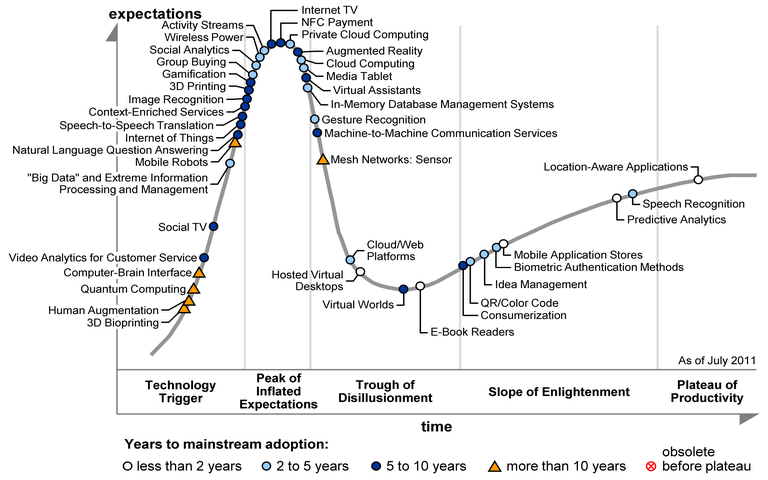
\includegraphics[width=0.75\textwidth]{gartner.png}
    \caption{Gartner Hype Cycle 2011 graphic}
    \label{fig:gart}
  \end{center}
\end{figure}

Despite being a term commonly referred, there is already criticism of gamification in the media. Some say that the term is a mere buzzword, applied as a simple "pointification", and often missing game elements such as storytelling and experiences, that are fundamental to the effectiveness of games.


\section{Existing work}

This section aims to introduce and analyse some existing services and applications related in some way to the concepts defined and explained in the previous sections of this chapter. This is particularly relevant because those concepts are behind the work meant to be developed in this thesis work and the project in which it is inserted.

\subsection{Social Networks for travellers}

In this chapter, it was already mentioned that there are 'themed' social networks, directed towards
people with particular interests or hobbies. 
There are also several online social networks aiming to promote the sharing of information between travellers. These platforms try to become a must see for those who are thinking of travelling, planning a particular trip, or want to find places to see in a particular journey or a comfortable place to spend the night during that journey.

Some examples of those platforms are \emph{WAYN} \footnote{\url{http://wayn.com}}, \emph{Tripatini} \footnote{\url{http://tripatini.com}}, \emph{Gogobot} \footnote{\url{http://gogobot.com}} and \emph{IgoUgo} \footnote{\url{http://igougo.com}}. They try to connect travellers and tour operators, using social networks.

\begin{figure}[h!]
  \begin{center}
    \leavevmode
    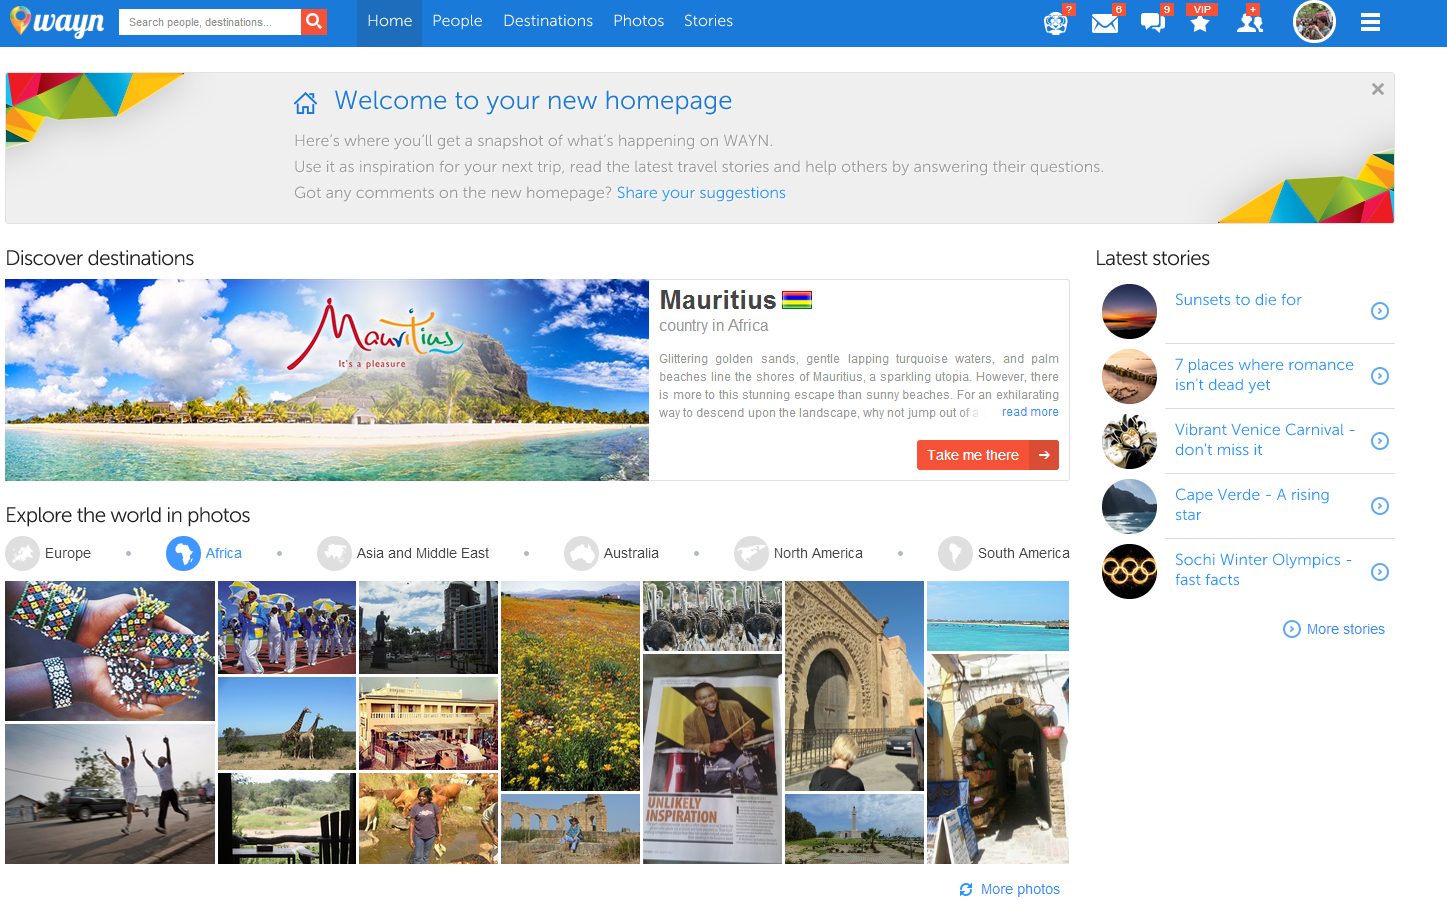
\includegraphics[scale=0.4]{wayn.png}
    \caption{Screenshot of \emph{WAYN} desktop interface}
    \label{fig:wayn}
  \end{center}
\end{figure}

However, these platforms have many disadvantages and do not represent what the implementation of the concept presented in \cite{kn:NGeCP11}. To start, these platforms aim to share information about long distance trips, in contrary to what is aimed to achieve (short-duration trips in a context of urban mobility).
Also, after a brief utilization and registration on some of those platforms, anyone can conclude that there is a strong presence of travel operators, filling up user's email accounts with messages, deals and offers to some destinations. 

A large percentage of the websites are also covered with those offers, turning the navigation and understanding of the platform very difficult and tiring, in what can be considered as a bad example of marketing utilization on online social networks, due to the excessive information that is presented.

Another problem of these platforms lies on the reliability of the information. In the end of 2009, a journalist named Arianne Cohen, tested the limits of these platforms by travelling to a foreign and unknown destination for her (in the particular case, Istambul), using only mobile applications and social media to receive information about places to see and where to spend the night. The resulting experience was disappoint in what concerns to these travel-themed platforms, as Arianne obtained most part of her positive experiences from contacting people through general-use platforms, such as \emph{Twitter}, \emph{Facebook} and \emph{Google+} \cite{kn:Coh10}.

\emph{Tripatini} presents us with yet another problem: usability and appearance. The platform's interface looks outdated and the existing information is not well-structured.

In addition to this social networks designed for travellers, some information about public transport can be found on general-use platforms, because public transport companies have realized about the potential the networks have to act as a way to get closer to their customers and daily users, communicating with them.
Nowadays, it is fairly common to find \emph{Facebook} and \emph{Twitter} pages from the companies, used to disseminate information about their services and interact more directly with the customers.
For instance, \emph{Metro do Porto} is present on both \emph{Facebook} \footnote{\url{http://www.facebook.com/MetroPorto?sk=wall}} and \emph{Twitter} \footnote{\url{https://twitter.com/\#!/metrodoporto}}, as well as \emph{STCP} \footnote{\url{http://www.facebook.com/STCPSA?sk=wall}} \footnote{\url{https://twitter.com/\#!/STCPServicos}}.

\subsection{Mobile Applications using Location-Based Services}

As said before, the increasing use of smartphones lead to the appearance of new and richer location-based services (concerning the amount of information they gather about users' location). Some successful online social networks based their business model or main features precisely on the capacity to track the location of their users.

Perhaps the most successful example of this kind is \emph{Foursquare} \footnote{\url{http://pt.foursquare.com/}}, who allows the 'check-in' of users at several locations (bars, restaurants, clubs, etc.), employing gamification techniques (badges) to improve user engagement with the network. The mobile application of the platform gathers the user location, giving him information about the nearest interest points, and allowing him to perform manual check-in at one of these locations.
A user earns a badge for completing tasks, such as checking-in for the first time at a new place, checking-in at a wide number of places in the same area, or several times in the same place. The platform also allows searching for particular categories of points of interest, and check the places visited by an user acquaintance.

\begin{figure}[h!]
  \begin{center}
    \leavevmode
    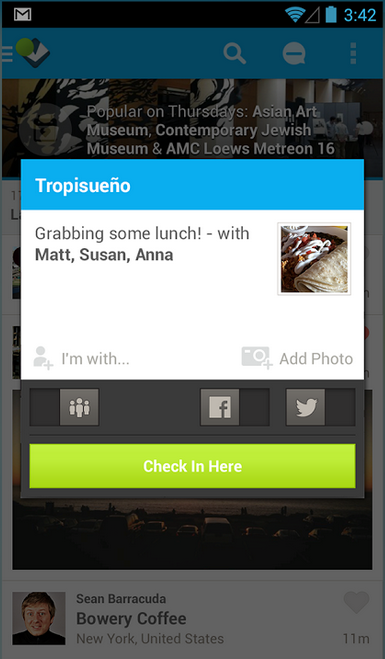
\includegraphics[scale=0.5]{foursquare.png}
    \caption{Screenshot of \emph{Foursquare} Android mobile application interface}
    \label{fig:fsqr}
  \end{center}
\end{figure}


\emph{Foursquare} had, as of February 2013, more than 40 million registered users, with several millions of check-ins registered in a daily basis.

Some other examples of successful online social networks that take advantage of the location of their users are \emph{Blendr} \footnote{\url{http://blendr.com/}} and \emph{Tinder} \footnote{\url{http://www.gotinder.com/}}. Their main goal is to, using that location, search for people nearby in order to arrange online dates between users.

\begin{figure}[h!]
  \begin{center}
    \leavevmode
    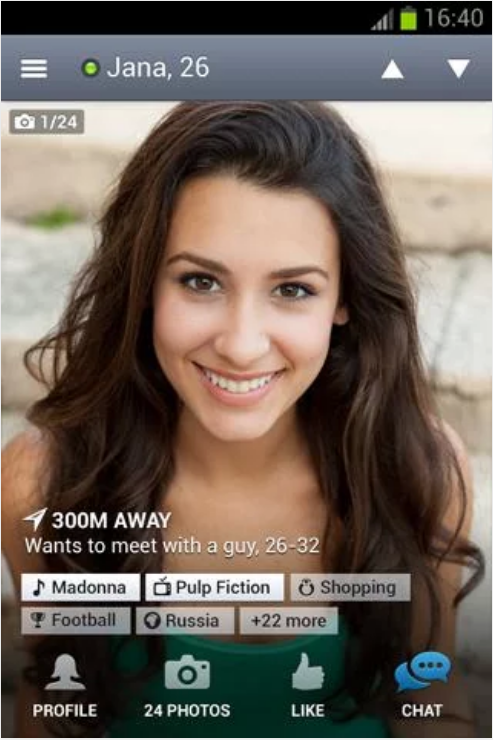
\includegraphics[scale=0.5]{blendr.png}
    \caption{Screenshot of \emph{Blendr} Android mobile application interface}
    \label{fig:blndr}
  \end{center}
\end{figure}

\emph{Tinder}, for instance, provides users with a sort of catalog from other users nearby, prompting them with a choice: marking them as a possible interest or not. Then, if the other person does the same thing, communication between the two users is enabled. 

\begin{figure}[h!]
  \begin{center}
    \leavevmode
    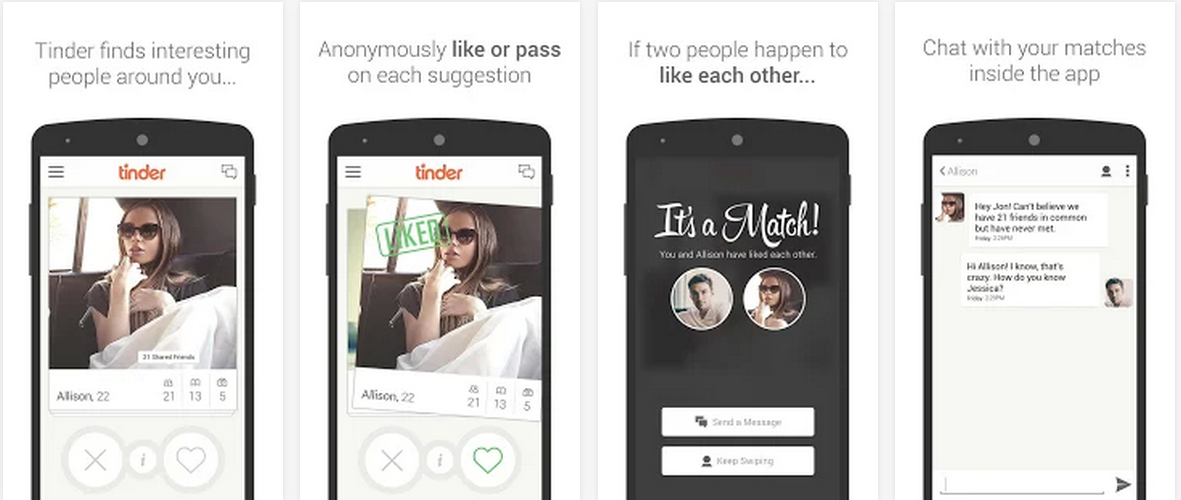
\includegraphics[width=0.75\textwidth]{tinder.png}
    \caption{Workflow of \emph{Tinder} application interface}
    \label{fig:tindr}
  \end{center}
\end{figure}

These two social networks, along with similar applications, demonstrate how a location-based service can be used in a context where the location of nearby users is deeply explored, and the number of existing users a critical factor for their success.

\pagebreak

\subsection{Route Planners}

Route planning services consist in one of the most used services for those who want to plan a trip using the Internet, whether it is short or medium duration trips. 
These services are usually free of charge, and allow their users to view Earth's maps and satellite images, offering route planning features using several types of transportation (walking, by public transport or by private car). They are particularly useful to find the shortest or fastest route between two given points. 
The most known service of this type is \emph{Google Maps}, but there are some alternatives, such as \emph{MapQuest} or \emph{Bing Maps}.

Given their features, these services normally have a simple and intuitive interface, making them easy to interact with.

\subsection{Mobile Applications for Public Transport}

In the last few years, some public transport companies tried to provide their users some valuable information about their services. That resulted in several applications, spread by a lot of countries and cities.

Some of those applications are: \emph{London Underground} \footnote{\url{https://play.google.com/store/apps/details?id=com.visualit.tubeLondonCity&hl=pt_PT}}, \emph{Catch that Bus!} \footnote{\url{https://play.google.com/store/apps/details?id=uk.co.ashtonbrsc.catchthatbus}}, \emph{National Rail Enquiries} \footnote{\url{https://play.google.com/store/apps/details?id=uk.co.nationalrail.google}}, \emph{iMetroPorto} \footnote{\url{https://play.google.com/store/apps/details?id=pt.edgelabs.metro_porto}} and \emph{MOVE-ME} \footnote{\url{https://play.google.com/store/apps/details?id=com.moveme}}.

\begin{figure}[h]
\begin{center}
\leavevmode
\subfloat[\emph{Catch That Bus!}]{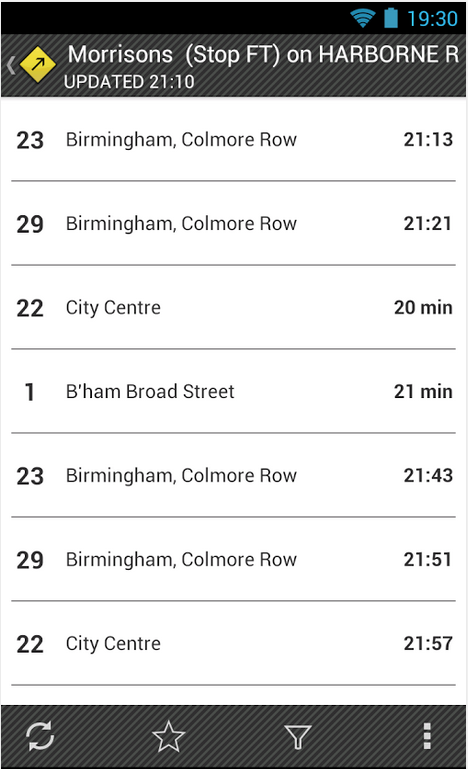
\includegraphics[width=2.5in]{catch.png}} \hspace{1em}%
\subfloat[\emph{London Underground}]{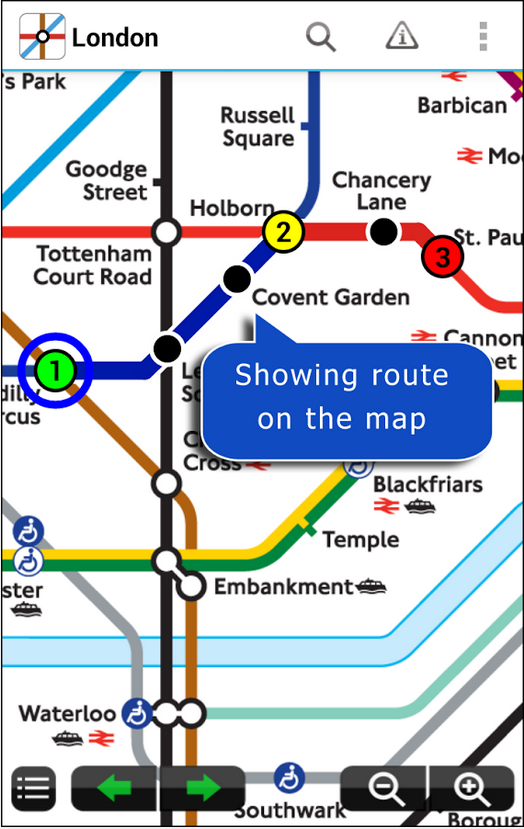
\includegraphics[width=2.5in]{london.png}}
\caption{Interfaces of mobile applications for public transport information - Example 1}
\label{fig:interfaces1}
\end{center}
\end{figure}

\begin{figure}[h]
\begin{center}
\leavevmode
\subfloat[\emph{National Rail Enquiries}]{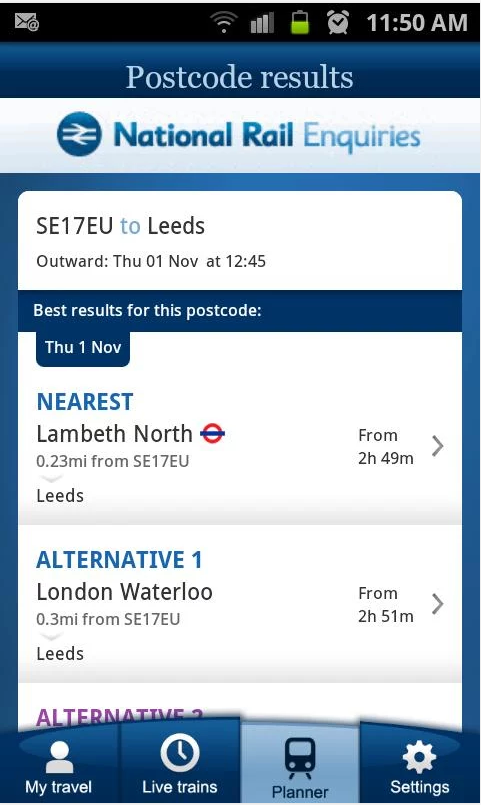
\includegraphics[width=2.5in]{national.png}} \hspace{1em}%
\subfloat[\emph{MOVE-ME}]{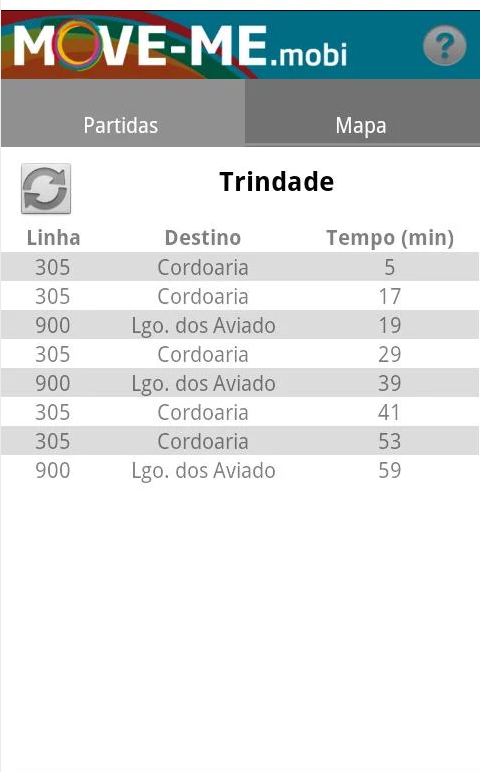
\includegraphics[width=2.5in]{moveme.png}}
\caption{Interfaces of mobile applications for public transport information - Example 2}
\label{fig:interfaces2}
\end{center}
\end{figure}



In the range of features provided by these applications, it is possible to find: 

\begin{itemize}
\item Information about schedules, lines and upcoming vehicles in real time.
\item Journey planner features.
\item Current location and nearest train/underground stations or bus stops.
\end{itemize}

There are, however, some disadvantages to this sort of mobile applications. They are usually limited to a city or urban area, or even to a specific method of transport, constraining their usage and potential.
The existing journey planner features, are in most cases pretty limited, not showing warnings or notifications to the users about delays or other events in the planned journey (only \emph{National Rail Enquiries} informs travellers about delays or cancelled trains).

Another downside of these applications, however not visible to the travellers, is that they rely on an existing API in the company's servers. To provide information of this kind to their clients, a public transport company must support the costs of developing and maintained such solution, costs that can be avoided if an application using crowdsourcing (where the information originates in the users themselves) is available in the said urban areas.

\subsection{Mobile Applications with Crowdsourcing}

Starting from the last constraint mentioned in the last set of existing applications, there has been developments in recent years in order to launch new solutions based on crowdsourcing, where users can access detailed information that were previously generated by other users. The potential of this type of applications is tremendous, specially in areas where there are many users  constantly using the application, receiving and submitting information possibly useful to other people with the same intentions. 
Obviously, transportation in urban areas is a field where this potential can be explored, giving the amount of people using private or public transport in a daily basis and sharing travel intentions.

That has lead to the appearance of platforms such as \emph{Waze} \footnote{\url{https://www.waze.com/}} and \emph{Moovit} \footnote{\url{http://www.moovitapp.com/}},  that are the closest existing applications compared to the project in which this thesis work is inserted.
\emph{Waze} is directed towards private transportation, feeding users with information about traffic and navigation provided by other users of the platform. Drivers can also report traffic issues, such as traffic jams or accidents, in order to warn other drivers, giving them the possibility to act accordingly with the situation.

\begin{figure}[h]
\begin{center}
\leavevmode
\subfloat[Route information]{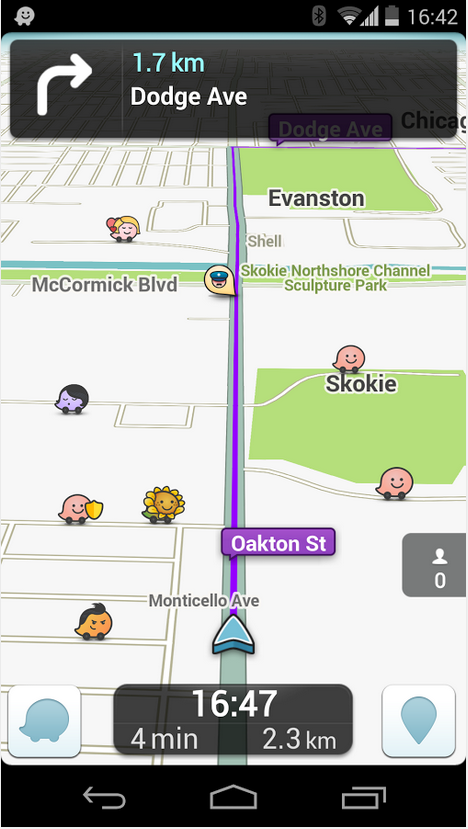
\includegraphics[width=2.5in]{waze1.png}} \hspace{1em}%
\subfloat[Report feature]{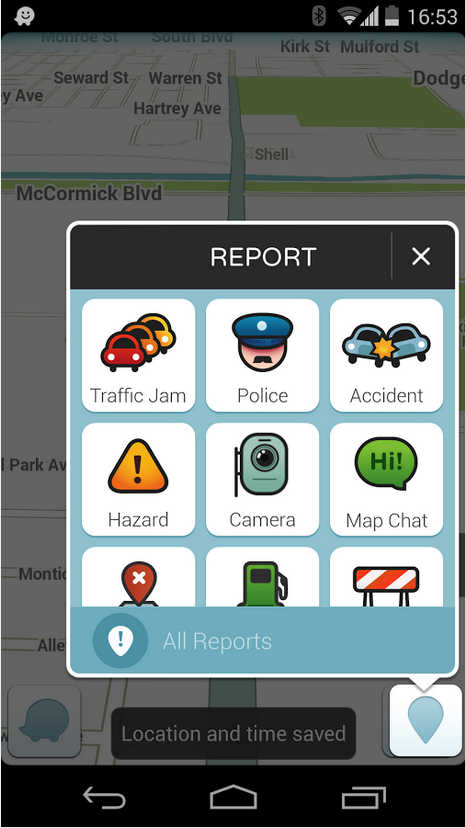
\includegraphics[width=2.5in]{waze2.png}}
\caption{Captions of \emph{Waze} mobile application interface.}
\label{fig:waze}
\end{center}
\end{figure}

\emph{Moovit}, however, is directed towards public transportation, feeding users with information about schedules in real time, re-routing in case of  delays, and also about crowding level of the vehicle.
The information provided is generated by and shared between other users, thus making \emph{Moovit} the most similar platform to this project's concept (however, it still does not take into account other aspects of the trip that we aim to see shared between users).

\begin{figure}[h]
\begin{center}
\leavevmode
\subfloat[\emph{Trip information feature.}]{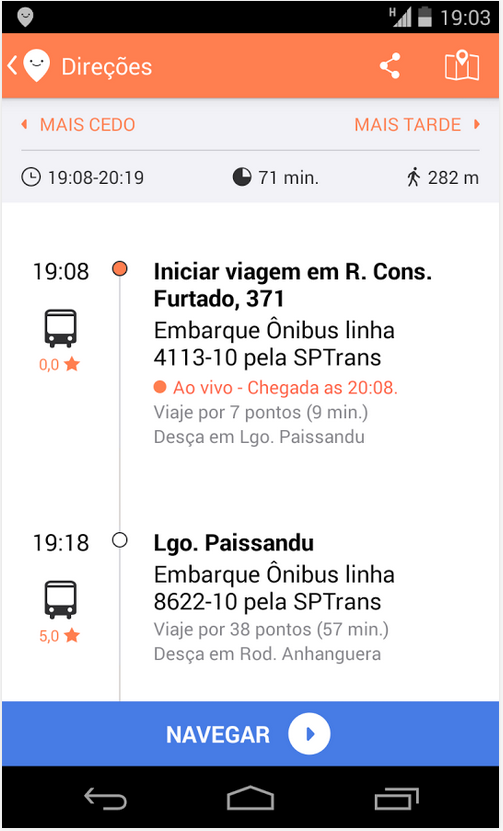
\includegraphics[width=2.5in]{moovit1.png}} \hspace{1em}%
\subfloat[\emph{Report information feature.}]{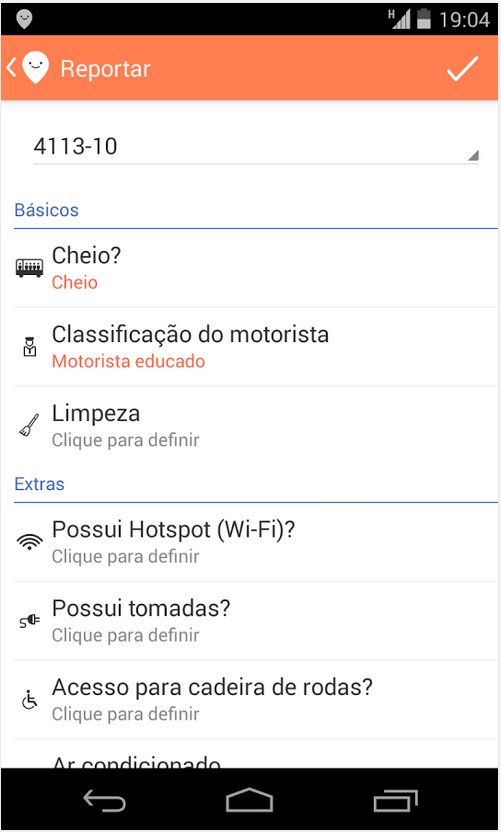
\includegraphics[width=2.5in]{moovit2.png}}
\caption{Captions of \emph{Moovit} mobile application interface.}
\label{fig:moovit}
\end{center}
\end{figure}

A final note about the interface of both these applications: after a brief use, the interfaces seemed very attractive, but not exactly clear to the user in what the buttons in the interface are meant to do or show.

\section{Summary}

After the literature review and a study of existing applications, it is concluded that there are good examples of services that use location of users and gamification techniques to improve user engagement, and that some of those aspects can be used in the interface meant to be developed in this thesis work. 

Concerning applications directed for public transport information, besides the limitations already mentioned, there are no applications feeding users with the information this project desires to provide them with. Also, because the final desired prototype is not limited to show information to the users, but also to make the task of sharing and submitting information as simple as possible, the usability of the application gains much more importance compared to the other existing applications in the field.